\documentclass[manuscript,screen]{acmart}

\usepackage{pgfplots}
\usepackage{caption}
\usepackage{subcaption}

\AtBeginDocument{%
  \providecommand\BibTeX{{%
    \normalfont B\kern-0.5em{\scshape i\kern-0.25em b}\kern-0.8em\TeX}}}

\setcopyright{acmcopyright}
\copyrightyear{2019} 
\acmYear{2019} 
\setcopyright{acmlicensed}
\acmConference[PEARC '19]{Practice and Experience in Advanced Research Computing}{July 28-August 1, 2019}{Chicago, IL, USA}
\acmBooktitle{Practice and Experience in Advanced Research Computing (PEARC '19), July 28-August 1, 2019, Chicago, IL, USA}
\acmPrice{15.00}
\acmDOI{10.1145/3332186.3333056}
\acmISBN{978-1-4503-7227-5/19/07}

%% Submission ID.
%% Use this when submitting an article to a sponsored event. You'll
%% receive a unique submission ID from the organizers
%% of the event, and this ID should be used as the parameter to this command.
%%\acmSubmissionID{123-A56-BU3}

\begin{document}

\title{Mii: An Automated Search Engine for Environment Modules}

\author{Justin Stanley}
\email{jtst@iastate.edu}
\affiliation{%
  \institution{Iowa State University}
  \city{Ames}
  \state{Iowa}
  \postcode{50010}
}

\begin{abstract}
The use of environment modules in HPC systems is rapidly gaining traction due to the increasing complexity of
managing research software. While environment modules improve organization for administrators, they can be
unfriendly to end-users, especially those less familiar in UNIX-like shell environments. I created a search engine for
modules that allows users to query available modules by the names of the commands they provide. Furthermore,
I wrote integrations for the popular shells \texttt{bash} and \texttt{zsh} that completely automate the searching and the loading
process.
\end{abstract}

\begin{CCSXML}
<ccs2012>
<concept>
<concept_id>10003120.10003121.10003124.10010862</concept_id>
<concept_desc>Human-centered computing~Command line interfaces</concept_desc>
<concept_significance>500</concept_significance>
</concept>
</ccs2012>
\end{CCSXML}

\ccsdesc[500]{Human-centered computing~Command line interfaces}

\keywords{HPC, modules, accessibility}

\maketitle

\section{Introduction}
Environment modules allow users to dynamically load and unload software into their working environment.
Often, a module will introduce a new command into the user’s shell. This is accomplished by modifying
the \texttt{PATH} environment variable that is scanned by the operating system when the user tries to execute a
command. However, the module rarely contains any metadata about \textit{which} commands it will make accessible
to the user once it is loaded. As a result, if the user needs to execute a certain command but does not
know the name of the module which provides it, they must contact the system administrator to receive the
module name. This is a less-than-optimal user experience and could be improved by tracking more relevant
information about modules.

\par

Making module environments more friendly and interactive will save both users and administrators much
time and frustration. Users will struggle less at the command line and administrators can dedicate their
time to more important matters.

\par

To store more information about modules, each available module file must be analyzed. Modules can affect
the environment in several ways. It can be difficult to predict how changes to environment variables will
affect the execution of programs. Also, loading modules can be quite expensive; often a module will depend
on many others, forming a tree of modules which all must be loaded first. This can cause loading individual
modules to take several seconds, making loading every available module infeasible in a timely manner.
As a result, the indexing tool must analyze the properties and effects of module files without actually loading
them.

\par

While the concept of environment modules has been around since 1991 \cite{TclPaper}, it is still steadily gaining
popularity in HPC systems. User issues with modules are relatively easy for an administrator to solve; the
user likely knows the name of the tools they are looking for and the administrator only needs to inform
them of the module name which provides it.

\par

\textit{Mii} constructs a local database of modules and their behaviors. The indexer walks through the user’s
\texttt{MODULEPATH} and finds module files. The module analyzer then infers the type of the module file and tries to
extract potential modifications to the \texttt{PATH} variable. \textit{Mii} then traverses through all of the potential \texttt{PATH}s
and looks for programs that the user is able to execute. Then, for each program found a row is inserted
into the local database associating the module file with the command it provides. Once the database is
constructed, \textit{Mii} is able to search for modules by command names.

\subsection{Primary features and benefits}

Once \textit{Mii} is installed for a user it will:
\begin{itemize}
\item Construct an index from binary names to module names
\item Hook into the shell, automatically loading modules when needed
\item Provide users with help and suggested commands
\end{itemize}

\section{Preliminaries}

There are currently two major implementations of environment modules. \textit{Environment Modules} \cite{TclPage} is
the implementation derived from the original work introducing the concept of environment modules \cite{TclPaper}.
\textit{Lmod} \cite{LmodPage} is a Lua-based successor to Environment Modules with a variety of improvements. Both of these
systems allow administrators to create \textit{module files} that define modifications to a user’s environment. These
modifications usually enable some collection of software to be accessible to the user once applied. This
method of dynamically loading software when needed instead of installing it globally greatly benefits software
organization and minimizes conflicts between software installations. It also enables multiple versions of a
software package to be installed at a time, allowing users to load any installed version they need.

\section{Concept and Usage}

Consider a researcher trying to use the popular \texttt{NCBI BLAST} search tool on her organization’s cluster. She
has a tutorial providing instructions on the \texttt{blastx} command. The cluster has an \textit{Lmod} installation
available to the users, with the \texttt{MODULEPATH} environment variable already correctly configured by the administrators.

\subsection{Module Autoloading}

If the researcher is unfamiliar with module-based systems, she might try and execute \texttt{blastx (...)} and
receive an error: \texttt{blastx: command not found}. Now, if she is aware of the environment module system she
might try and load the module by executing \texttt{module load blast}. However, this is not the correct module
name and she will receive another error: \texttt{(...) the following module(s) are unknown: "blast"}. At this
point the friendly administrator is contacted who informs her the correct way to load the blast module is
\texttt{module load blast-plus}. Finally the researcher loads the module and is able to use the \texttt{blastx} tool as
expected.

\par

\textit{Mii} eliminates this problem and makes loading modules more friendly and automated. Consider the same
scenario as before, except now \textit{Mii} is installed on the system with shell integration enabled. If the researcher
is unfamiliar with module-based systems she might execute \texttt{blastx (...)}. The \texttt{blast-plus} module is
not loaded so the shell is unable to execute the binary directly. Instead the shell-specific “command not
found” hook is called with the command information. Here \textit{Mii}’s shell integration intercepts the failure
and searches for modules that provide the \texttt{blastx} command. The \textit{Mii} search responds with an available
module \texttt{blast-plus}. As only one version of this module is installed on the system, it is immediately loaded
and the original command is re-executed with the original arguments. Our researcher sees \textit{Mii}’s response
before \texttt{blastx} is executed as originally intended: \texttt{[mii] autoloading blast-plus/2.7.1}. In the event that
multiple versions of \texttt{blast-plus} were available as modules, the researcher would be prompted to select a
version before proceeding with the command.

\subsection{Fuzzy Searching}

\textit{Mii} also supports fuzzy searches. When the researcher executes the command \texttt{BlastX}, \textit{Mii} is unable to find
any modules that provide the command. The database is then searched for similar-looking commands, and
the researcher receives a suggestion: \texttt{[mii] hint: try a similar command ‘blastx’ ‘tblastx’} indicating
the correct command to execute.

\subsection{Implementation Details}

\textit{Mii} currently reconstructs its database whenever the user logs into a shell. This ensures that the module index is
always up to date with the installed modules on the system. \textit{Mii} is written in POSIX-compliant C and uses
\textit{SQLite 3} to store the module index. The search engine is designed to have minimal dependencies and to be
easy to deploy into an existing system. Integration scripts are shell-specific and must be written for each
supported shell. I only wrote scripts for \texttt{bash} and \texttt{zsh} but any shell with a command-not-found hook can be
supported.

\section{Performance Experiments}

I conducted extensive performance testing with the \textit{Mii} environment \cite{MiiPage}, analyzing the speed of building the
database as well as querying it. As \textit{Lmod} module files are scanned in a different manner than \textit{Environment Modules (Tcl)}
module files separate data was collected for each module type.

\section{Analysis}

\begin{figure}
    \centering
    \begin{subfigure}{.5\textwidth}
        \centering
        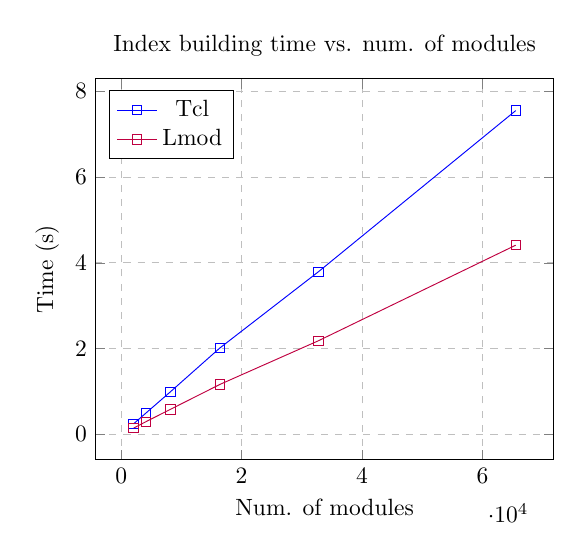
\begin{tikzpicture}[scale=0.85]
            \begin{axis}[
                title={Index building time vs. num. of modules},
                xlabel={Num. of modules},
                ylabel={Time (s)},
                legend pos=north west,
                grid=major,
                grid style=dashed,
            ]

            \addplot[
                color=blue,
                mark=square,
            ]
            coordinates {
                (2048, 0.24)(4096, 0.49)(8192, 0.99)(16384, 2.01)(32768, 3.79)(65536, 7.55)
            };
            \addlegendentry{Tcl}

            \addplot[
                color=purple,
                mark=square,
            ]
            coordinates {
                (2048, 0.14)(4096, 0.29)(8192, 0.58)(16384, 1.16)(32768, 2.18)(65536, 4.41)
            };
            \addlegendentry{Lmod}

            \end{axis}
        \end{tikzpicture}
    \end{subfigure}%
    \begin{subfigure}{.5\textwidth}
        \centering
        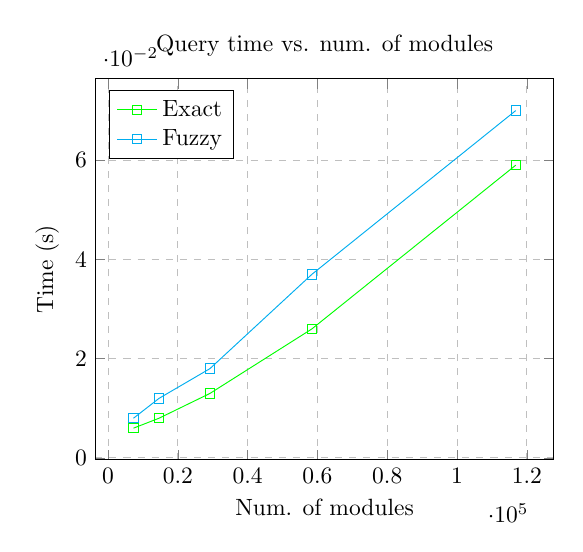
\begin{tikzpicture}[scale=0.85]
            \begin{axis}[
                title={Query time vs. num. of modules},
                xlabel={Num. of modules},
                ylabel={Time (s)},
                legend pos=north west,
                grid=major,
                grid style=dashed,
            ]

            \addplot[
                color=green,
                mark=square,
            ]
            coordinates {
                (7300, 0.006)(14600, 0.008)(29200, 0.013)(58400, 0.026)(116800, 0.059)
            };
            \addlegendentry{Exact}

            \addplot[
                color=cyan,
                mark=square,
            ]
            coordinates {
                (7300, 0.008)(14600, 0.012)(29200, 0.018)(58400, 0.037)(116800, 0.070)
            };
            \addlegendentry{Fuzzy}

            \end{axis}
        \end{tikzpicture}
    \end{subfigure}
    \caption{Performance graphs}
    \label{fig:graphs}
\end{figure}

\begin{table}
  \begin{tabular}{ccc}
    \toprule
      Num. modules & Lmod time (s) & Tcl time (s) \\
    \midrule
      2048 & 0.14 & 0.24 \\
      4096 & 0.29 & 0.49 \\
      8192 & 0.58 & 0.99 \\
      16384 & 1.16 & 2.01 \\
      32768 & 2.18 & 3.79 \\
      65536 & 4.41 & 7.55 \\
  \bottomrule
\end{tabular}
  \caption{Index building time data}
  \label{tab:build}
\end{table}

\begin{table}
  \begin{tabular}{ccc}
    \toprule
      Num. modules & Exact query time (s) & Fuzzy query time (s) \\
    \midrule
      7300 & 0.006 & 0.008 \\
      14600 & 0.008 & 0.012 \\
      29200 & 0.013 & 0.018 \\
      58400 & 0.026 & 0.037 \\
      116800 & 0.059 & 0.070 \\
  \bottomrule
\end{tabular}
  \caption{Query time data}
  \label{tab:search}
\end{table}

The index building performance data from figure \ref{fig:graphs} indicates that \textit{Lmod} modules are significantly faster to
index than \textit{Tcl} modules. This is to be expected as the \textit{Lmod} analysis method executes a simple regular
expression on the module file while the \textit{Tcl} analysis method must simulate the whole file. This is because
Tcl modules can contain variable expansions in the \texttt{PATH} variables which requires a more expensive analysis.
Both the searching and indexing performance appear to execute in linear time which is to be expected.

\section{Conclusions}

In summary, \textit{Mii} has been developed to be a useful extension to an existing module-based system. Based
on the performance analysis \textit{Mii} is fast enough to be integrated with most existing systems without any
noticeable performance impact. The \textit{Mii} engine introduces a new type of module interaction and interactive
user experience.

\par

\textit{Mii} is free and open-source software \textit{(MIT)}, hosted publicly at \url{https://github.com/codeandkey/mii}. Contributions are welcomed and encouraged!

\section{Future Work}

While \textit{Mii} is in a working state and accomplishes its primary goal, there is still much room for improvement
and new features. \textit{Mii} does not take advantage of multithreaded systems, which could radically improve the
index building performance. Also, rebuilding the module index on every login is often unnecessary; perhaps
another trigger could be introduced that would only rebuild the index when modules are added or removed.
\textit{Mii} currently only indexes modules by binaries provided in their \texttt{PATH}s. The index could be expanded to
store even more relevant module information for other uses, such as manual pages provided in \texttt{MANPATH}s.
\textit{Mii}’s shell integration could then be further expanded to automatically load modules for missing manual
pages.

\par

There is currently a refactoring effort underway to reimplement the \textit{Mii} engine in the modern \textit{Rust} language.
The refactor will introduce a differential indexing system as well as a multithreaded architecture.

\begin{acks}
Thanks to Levi for introducing me to HPC and Miles for the moral support!
\end{acks}

\bibliographystyle{ACM-Reference-Format}
\bibliography{mii}

\appendix
\section{Performance Data}
For performance data please refer to tables \ref{tab:build} and \ref{tab:search}. Graphical analyses are shown in figure \ref{fig:graphs}.

\end{document}
\endinput
